\documentclass{article}
\usepackage[utf8]{inputenc}
\usepackage{listings}
\usepackage{amsfonts}
\usepackage{enumerate}
\usepackage[a4paper, total={7in, 10in}]{geometry}
\usepackage{xcolor}
\usepackage{multicol}
\usepackage[compact]{titlesec}
    \titlespacing{\section}{0pt}{2ex}{2ex}
    \titlespacing{\subsection}{0pt}{2ex}{2ex}
\usepackage{hyperref}
\usepackage{graphicx}
\usepackage{float}
    
\lstdefinestyle{mystyle}{
    backgroundcolor=\color{white},   
    commentstyle=\color{blue},
    keywordstyle=\color{red},
    numberstyle=\tiny\color{black},
    stringstyle=\color{black},
    basicstyle=\ttfamily\footnotesize,
    breakatwhitespace=false,         
    breaklines=true,                 
    captionpos=b,                    
    keepspaces=true,                 
    numbers=left,                    
    numbersep=5pt,                  
    showspaces=false,                
    showstringspaces=false,
    showtabs=false,                  
    tabsize=2
}
\lstset{style=mystyle}





\title{Assignment2}
\author{tamajoalberto }
\date{May 2020}

\begin{document}

\begin{titlepage}
        \begin{center}
        
            \vfill
            \Huge
            \textbf{COMP1204\\}
            
            
            Coursework 2\\
        
            \vfill
            
            \textbf{Alberto Tamajo\\}
            \vspace{1cm}
            \Large
            Student ID: 30696844
            \vfill
            May 2020\\
            Electronics and Computer Science Department\\
            University of Southampton\\
        \end{center}
    \end{titlepage}
\section{Introduction}
The dataset provided in the coursework description has been manipulated as an already-built RELATION in order to perform the Normalisation Section. However, the relations schema resulting from the normalisation steps are definitely not sensible relations that can be used in a real-life database. Indeed, a real-life database that stores the information contained in the dataset provided would have the following relations schema:\\
\begin{itemize}
    \item Countries(ID,countriesAndTerritories,geoId,countryTerritoryCode, popData2018, ContinentID)
    \item Continents(ID, continentExp)
    \item Reports(dateRep, cases, deaths, CountryID)
\end{itemize}
The relations schema above come from the fact that in the E/R model that represents the data contained in the provided dataset there would be three entities (Countries, Continents and Reports) where Reports is also a WEAK ENTITY as its key comprises the key of Countries. Reports contains the primary key of Countries (ID) because there exists a many-to-one relationship from Reports to Countries. Countries has a surrogate key (ID) because this way it is possible to resolve the problem of the NULL values on the countryTerritoryCode column. 
In conclusion, I have written this introduction section to posit that I did the best possible to create a database that would be used in a real-life context. However, it has turned out that it is not possible because of the fact that the dataset that has been provided had to be considered as an already-built relation, otherwise, it wouldn't be possible to perform section 2 of the coursework because the relation schemas resulting from the E/R diagram based on the dataset would already be normalised. Consequently, it is not possible to fully consider the domain and future data of the dataset as this would lead not to perform the whole section on normalisation. 
 
\section{The Relational Model}
\subsection{EX1}

 The relation in the dataset is an 11-ary relation which can be represented mathematically in the following way( assuming the name of the relation is Coronavirus):
\begin{center}
    

\textbf{Coronavirus $\subseteq$ dateRep $\times$ day $\times$ month $\times$ year $\times$ cases $\times$ deaths $\times$ countriesAndTerritories $\times$ geoId $\times$ countryterritoryCode $\times$ popData2018 $\times$ continentExp}
\end{center}
The schema of the relation is the following(assuming no tuples about the international conveyance are present):
\begin{center}
    
    \textbf{Coronavirus(dateRep : DATE, day : TINYINT, month : TINYINT, year : SMALLINT,\\ cases : INT, deaths : INT, countriesAndTerritories : VARCHAR(255), geoId : CHAR(2), countryterritoryCode : CHAR(3),  popData2018 : BIGINT, continentExp : VARCHAR(255))}.\\
    
\end{center}




The datatypes used above are included in SQL which is an an ANSI/ISO standard.
However, SQlite has a restricted set of data types compared to the SQL standard. Indeed, in SQlite (which uses a dynamic type system) each column can have only the following affinities:
\begin{center}
    \textbf{TEXT, NUMERIC, INTEGER, REAL, BLOB}
\end{center}
These affinities are used to build the relations schema in EX11.

\subsection{EX2}
    
 The MINIMAL BASIS of functional dependencies of the relation Coronavirus is provided below (it is possible to derive all possible functional dependencies of the relation from the MINIMAL BASIS): 
\begin{multicols}{2}
\begin{itemize}
    \item dateRep $\rightarrow$ day
    \item dateRep $\rightarrow$ month
    \item dateRep $\rightarrow$ year
    \item day,month,year $\rightarrow$ dateRep
    \item countriesAndTerritories $\rightarrow$ geoId
    \item geoId $\rightarrow$ countriesAndTerritories
    \item geoId $\rightarrow$ countryterritoryCode
    \item geoId $\rightarrow$ continentExp
    \item countryterritoryCode $\rightarrow$ popData2018
    \item dateRep,geoId $\rightarrow$ cases, deaths
     
\end{itemize}
\end{multicols}
In the appendix section \textcolor{blue}{\nameref{FS}} all functional dependencies derivable from the MINIMAL BASIS are outlined.
Trivially, dateRep functionally determines day, month, year and viceversa. dateRep and geoId functionally determine cases and deaths because there cannot be two different tuples with same values for dateRep and geoId and different number of cases and deaths. Furthermore, later it will be shown that dateRep and geoId is a candiate key of the relation and so there cannot exist two tuples with same values for dateRep and geoId.  
The attribute \textbf{geoId} is an ISO Alpha-2 Code while the attribute \textbf{countryterritoryCode} is an ISO Alpha-3 Code and both of them uniquely identify a country. Therefore, it follows that geoId functionally determines countriesAndTerritories, countryTerritoryCode, popData2018 and continentExp. However, even though countryTerritoryCode is an ISO Alpha-3 Code, in the dataset provided it functionally determines popData2018 but does not functionally determine countriesAndTerritories, geoId and continentExp because the countryTerritoryCode contains NULL values. NULL values are not values in themselves but are UNKNOWN values in a dataset. However, in this specific case all the values of the CountryterriotryCode are known as they are ISO Alpha-3 Codes. Therefore, the optimal solution would be to fill the NULL values with the correct values and in a real life context this problem would be easily resolved this way and CountryTerritoryCode would be a prime member. Nonetheless, I won't do so because otherwise there wouldn't be transitive dependencies and I could not solve EX7 and EX8. Thus, I will treat the countryTerritoryCode as an UNKNOWN column whose meaning is not known (pretending it is not an ISO Alpha-3 Code). Since, the countryterriotryCode contains NULL values and the meaning of the column is not known then the only reasonable thing to do is to check whether it is possible to create \textbf{realisable} functional dependencies under null markers from the countryterritoryCode attribute by just inspecting the data provided.

It turns out that it is possible to create only the following  \textbf{realisable} functional dependency:\\ countryterritoryCode $\rightarrow$ popData2018\\
For example, It would be incorrect to consider \textbf{countryterritoryCode $\rightarrow$ continentExp} as a functional dependency (even though countryterritoryCode is an Alpha-3 Code) because the provided dataset  contains null values in the countryterritoryCode column and the continentExp column does not contain null values. Therefore, this functional dependency is not \textbf{realisable} under null markers because it is not possible to replace all null markers with a certain value without violating the FD itself.
An example will clarify what has been said above.
In the provided dataset  there exists a row where the countryterritoryCode value is null and the continentExp value is "America". In addition, there exists also a row where the countryterrytoryCode value is null and the continentExp value is "Africa". If we replaced the null values with an arbitrary value x then the functional dependency wouldn't hold because it is not true that \textbf{countryterritoryCode $\rightarrow$ continentExp} as there exist 2 rows where the value of the countryterritoryCode is x but the continentExp values are different. In conclusion, the FD \textbf{countryterritoryCode $\rightarrow$ continentExp} is not realizable and for similar reasons also \textbf{countryterritoryCode $\rightarrow$ geoId} and \textbf{countryterritoryCode $\rightarrow$ countiresAndTerritories} \textcolor{blue}{(Antonio Badia, Daniel Lemire, Functional Dependencies with null Markers, The Computer Journal, Volume 58, Issue 5, May 2015, Pages 1160–1168)}. 

On the other hand, \textbf{countryterritoryCode $\rightarrow$ popData2018} is a realisable functional dependency because whenever the value of the countryterritoryCode is null, the value of the popData2018 is null as well. Thus, it is possible to replace the null values of the countryterritoryCode column and the popData2018 column with arbitrary values x and y respectively and the functional dependency would hold nonetheless. In some cases, the value of the column countryterritoryCode is not null but the value of the popData2018 is null. Also in this case the functional dependency trivially holds.\\
All the functional dependencies will hold also in the future by enforcing that the following attributes cannot have null values: dateRep, day, month, year, countriesAndTerritories, geoId.
I really want to stress that this is not what I would do in real-life because it would be enough to fill the null values with known values. However, I didn't do so because otherwise I could not perform EX7 and EX8. Additionally, it makes sense to look for realisable functional dependencies from the countryterriotryCode because I have said that I treated the column as a column whose meaning is not known and can be inferred just by inspecting the dataset provided.
\subsection{EX3}
 From the MINIMAL BASIS is possible to detect the following potential candidate keys:
 \begin{multicols}{2}
\begin{itemize}
    \item (dateRep, countriesAndTerritories)
    \item (dateRep, geoId)
    \item (day, month, year, countriesAndTerritories)
    \item (day, month, year, geoId)
\end{itemize}
\end{multicols}
It is possible to prove that they are keys by taking the closure of each of them. However, taking the closure of each them does not guarantee that they are minimal keys. By taking the closure of any proper subset of each of them leads to the fact that none of the proper subsets of each of them is a key, thus they must me minimal keys. CountryTerritoryCode is not a prime member in the provided dataset because of the NULL values.
\subsection{EX4}
 The chosen primary key is the following:
\begin{itemize}
    \item (dateRep, geoId)
\end{itemize}
(dateRep, geoId) has been chosen over the other candidate keys because it is the key with the least number of attributes and because geoId is an ISO ALPHA-2 Code which uniquely identify every country internationally. Thus, the attribute geoId is not likely to change and is language-independent as well.
\section{Normalisation}
\subsection{EX5}
\begin{itemize}
    \item countriesAndTerritories $\rightarrow$ countryterritoryCode, popData2018, continentExp
    \item geoId $\rightarrow$ countryterritoryCode, popData2018, continentExp
\end{itemize}
The relation is not in the Second Normal Form. In order to convert it into the Second Normal Form, it must be decomposed into two relations (CoronavirusCases, Country) such that:
\begin{itemize}
    \item CoronavirusCases = $\Pi_{dataRep, \:day, \:month, \:year, \:cases, \:deaths, \:countriesAndTerritories, \:geoId}(Coronavirus)$
    
    \item Country = $\Pi_{geoId,\: countryterritoryCode,\: popData2018,\: continentExp}(Coronavirus)$
    
\end{itemize}
\textcolor{blue}{\nameref{EX5}} for additional details.

\subsection{EX6}
The answer provided above exactly describes how to convert the relation Coronavirus into the Second Normal Form by decomposing it into two relations whose schema is described by the two linear algebra expressions.
The schema of the two new relations is (using standard SQL data types):
\begin{center}
    \item \textbf{CoronavirusCases(dateRep : DATE , day : TINYINT, month : TINYINT, year : SMALLINT,\\cases : INT, deaths : INT, countriesAndTerritories : VARCHAR(255), geoId : CHAR(2))}
\end{center}
\begin{center}
        \item \textbf{Country(geoId : CHAR(2), countryterritoryCode : CHAR(3), popData2018 ; BIGINT,\\ continentExp : VARCHAR(255))}
\end{center}
The primary key of the relation Coronaviruscases is (dateRep,geoId). The primary key of the relation Country is (geoId).
\subsection{EX7}
The relation CoronavirusCases does not contain transitive functional dependencies.\\
However, the relation Country contains the following transitive functional dependency:
\begin{itemize}
    \item geoId $\rightarrow$ popData2018\\
    \textbf{because:}
    \item geoId $\rightarrow$ countryterritoryCode
    \item countryterritoryCode $\rightarrow$ popData2018
\end{itemize}
\textcolor{blue}{\nameref{EX7}} for additional details.



\subsection{EX8}
In order to obtain a set of relations which all are in the Third Normal Form, the relation Country must be decomposed into 2 relations (CountryContinent, CountryPopulation) such that:
\begin{itemize}
    \item CountryContinent = $\Pi_{geoId, \:countryterritoryCode, \:continentExp}(Country)$
    
    \item CountryPopulation = $\Pi_{countryterritoryCode,\: popData2018}(Country)$
    
\end{itemize}
The schema of the two new relations is the following:
\begin{center}
    
    \textbf{CountryContinent(geoId : CHAR(2), countryterritoryCode : CHAR(3), continentExp : VARCHAR(255))}
\end{center}
\begin{center}
    \textbf{CountryPopulation(countryterritoryCode : CHAR(3), popData2018 : BIGINT)}
\end{center}
The primary key of the CountryContinent relation is (geoId).\\
The primary key of the CountryPopulation relation is (countryterritoryCode).\\
\textcolor{blue}{\nameref{EX8}} for additional details.
\subsection{EX9}
 A relation R is in the Boyce-Codd Normal Form if given that S is the set of FDs of R then for every FD of S such that FD = $A_1,A_2,...,A_n \rightarrow B_1,B_2,...,B_n$ it follows that $A_1,A_2,...,A_n$ is either a key or a super key. Therefore, the relation CoronavirusCases is not in the Boyce-Codd Normal form because of the following functional dependencies:
\begin{multicols}{2}
\begin{itemize}
    \item dateRep $\rightarrow$ day, month, year
    \item day, month, year $\rightarrow$ dateRep
    \item countriesAndTerritories $\rightarrow$ geoId
    \item geoId $\rightarrow$ countriesAndTerritories
\end{itemize}
\end{multicols}
The relation CountryContinent is in the Boyce-Codd Normal Form.\\
The relation CountryPopulation is in the Boyce-Codd Normal Form.\\
\textcolor{blue}{\nameref{EX9}} for additional details.
\section{Modelling}
\subsection{EX10}The dataset.csv file has been imported in SQlite and the database has been dumped ad dataset.sql
\subsection{EX11}
Since the dataset contains information about the Coronavirus cases and deaths in an international conveyance in Japan, I opted to create an additional table called "CruiseShips" which contains the tuples of dataset.csv which refer to the international conveyance. I believe it is not consistent to store the information about the conveyance in the relations resulting from the normalisation of the provided dataset.\\
\textbf{Indexes created:}
\begin{itemize}
    \item An index on the \textbf{countriesAndTerritories} attribute of the CoronavirusCases table so that all the queries which involve select-from-where (condition on countriesAndTerritories) statements are sped up.\\
    There is no need to create an index on the primary key because the primary key is already indexed by
a cluster index. Indeed, the tuples are physically stored into ascending order with respect to the geoId
attribute. For the same reason there is no need of creating an index on geoId. It is important to notice
that no index has been created for the attributes (dateRep, day, month, year, cases, deaths) because the main advantage
of using indexes is to retrieve the position of the tuples that contain a certain attribute value by bringing
in main memory the least number of secondary memory pages as possible (in order to retrieve even a
single tuple from a table, a whole page must be fetched from secondary memory). However, the attributes
(dateRep, day, month, year, cases, deaths) are sparse over most pages (if not all of them).

\item An index on the \textbf{countryterritoryCode} attribute of the CountryContinent table so that all the queries which involve select-from-where (condition on countryterritoryCode) statements are sped up.\\
The geoId attribute is already indexed by the cluster index. It is not convenient to create an index for
the continentExp attribute because the values of this attributes are sparse over many different disk pages
(if not all of them).
\item  No indexes have been created in the CountryPopulation table because the primary key is already a cluster index and the popData2018 values are sparse over many
disk pages.
\end{itemize}
Additionally, 3 views have been created to make the last queries more readable.\\It is important to notice that creating useless indexes is counterproductive because not only they do not speed up retrieval operations but may also worse the time needed to retrieve information because a B-Tree or B*-Tree must be traversed and additional pages must be fetched from secondary memory because indexes are stored in secondary memory pages.\\
\textcolor{blue}{\nameref{EX11}} for additional details.\\
\textcolor{blue}{\nameref{EX11Advantages}} for details about how more efficient the database shown in the introduction set is.


\subsection{EX12}The ex12.sql file has been produced and the database has been dumped into dataset3.sql
\subsection{EX13} Both ex11.sql and ex12.sql work as expected



\section{Querying}
\subsection{EX14}
 SELECT SUM(cases) AS totalCases,SUM(deaths) AS totalDeaths\\ FROM CoronavirusCases;\\\\
 I have not included the cases and deaths in the cruise ship tuples as some of them contain negative values.
 \subsection{EX15}
SELECT dateRep,cases\\ FROM CoronavirusCases\\ WHERE geoId="UK"\\ ORDER BY dateRep;
\subsection{EX16}
SELECT continentExp,dateRep,SUM(cases) AS totalCases,SUM(deaths) AS totalDeaths\\
FROM CoronavirusCases t, CountryContinent q\\
WHERE t.geoId=q.geoId\\
GROUP BY q.continentExp, t.dateRep\\
ORDER BY t.dateRep;
\subsection{EX17}
SELECT t.countriesAndTerritories,(1.0*t.sumCases/q.popData2018*100) AS percentageCases,\\ (1.0*t.sumDeaths/q.popData2018*100) AS percentageDeaths\\
FROM casesAndDeathsByCountry t,populationCountry q\\
WHERE t.geoId=q.geoId;
\subsection{EX18}
SELECT countriesAndTerritories,(1.0*sumDeaths/sumCases*100) AS mortalityRate\\
FROM casesAndDeathsByCountry\\
ORDER BY mortalityRate DESC\\
LIMIT 10;
\subsection{EX19}
SELECT dateRep,SUM(deaths) OVER (ORDER BY dateRep) AS cumulativeDeaths,\\SUM(cases) OVER (ORDER BY dateRep) AS cumulativeCases\\
FROM unitedKingdom\\
ORDER BY dateRep;
\section{Extension}
\subsection{EX20}
I have plot the top 10 countries so that to have a nice and more readable graph by using a liner plot.

\newpage
\section{Appendix}
\subsection{The script}
\begin{lstlisting}[language=bash, caption={plot.sh},escapeinside={(*}{*)},label={lst:counreviews.sh}]
#!/bin/bash

cmd="SELECT DISTINCT countriesAndTerritories FROM CoronavirusCases GROUP BY geoId ORDER BY sum(deaths) DESC LIMIT 10"

cmd2="SELECT DISTINCT dateRep FROM CoronavirusCases ORDER BY dateRep"

`sqlite3 coronavirus.db "CREATE TABLE CumulationDeaths(dateRep NUMERIC, countriesAndTerritories TEXT, sumdeaths INTEGER, PRIMARY KEY(dateRep,countriesAndTerritories))WITHOUT ROWID"`

`sqlite3 coronavirus.db "INSERT INTO CumulationDeaths SELECT dateRep,countriesAndTerritories, SUM(deaths) OVER (PARTITION BY geoId ORDER BY dateRep) AS sumDeaths FROM CoronavirusCases"`

IFS=$'\n'
fqry=(`sqlite3 coronavirus.db "$cmd"`)
fqry2=(`sqlite3 coronavirus.db "$cmd2"`)

OUT=$(mktemp dataXXX --suffix=.dat)

printf "date" >> "$OUT"

for country in "${fqry[@]}"; do

    printf ",$country" >> "$OUT"

done

for date in "${fqry2[@]}"; do

	printf "\n$date" >> "$OUT"

	for country in "${fqry[@]}"; do

		sumDeaths=(`sqlite3 coronavirus.db "SELECT sumDeaths from CumulationDeaths where dateRep=\"$date\" AND countriesAndTerritories=\"$country\""`)

    		printf ",$sumDeaths" >> "$OUT"
	done
done

gnuplot -persist <<-EOFMarker
set datafile separator ","
set title "Cumulative deaths by top 5 countries and by date"
set terminal png  enhanced font "arial,18" fontscale 1.0 size 1920, 1080
set output 'graph.png'
set style data linespoint


set yrange [0:80000]
set grid
set xdata time
set timefmt "%Y-%m-%d"
set format x "%Y-%m-%d"
set xlabel "Date"
set ylabel "Cumulative Deaths"
set xtics "2019-12-31",648000,"2020-04-27"
set xtic rotate by -45 font "Arial,18" scale 0



plot "$OUT" using 1:2 title column,for [i=3:*] '' using 1:i title columnheader(i)

EOFMarker

rm  "$OUT"

`sqlite3 coronavirus.db "DROP TABLE CumulationDeaths"`

\end{lstlisting}
\subsubsection{How the script works}
Basically, what the script does is to create a single comma-separated file consisting of 11 columns such that the first column represents a date while the $n^{th}$+1 column represents the $n^{th}$ country with the highest number of cumulative deaths up to the $27^{th}$ of April. The value contained in the $n^{th}+1$ column and $r^{th}$ row is the cumulative number of deaths of the $n^{th}$ country up to the $r^{th}$ date. Naturally, the dates are ordered into ascending order. The data contained in the file is plotted by using gnuplot which produces a file called graph.png.
\subsubsection{How all this is done}
From line 7 to line 9, a table called Cumulationdeaths is created in the coronavirus database and is populated with tuples containing the following information in the same exact order: date, country name, sum of cumulative death of the country up to the given date. Naturally, this information is extracted from the CoronavirusCases table.
The new table CumulationDeaths is mainly created to speed up the process of creating the comma-separated file as using a view would only make the successive queries in the script cleaner but not very efficient because the data of the table would not be physically stored. The attributes dateRep and countriesAndTerritories are the primary key of the CumulationDeaths table and this will help extensively in the successive queries in the script because they extract information based on both attributes and SQLite creates automatically a cluster index on both of them.\\
In line 12, the variable \textbf{fqry} is an array containing the top 10 countries with the highest number of cumulative deaths up the $27^{th}$ of April (the countries are ordered into a descending order in the array).\\
In line 13, the variable \textbf{fqry2} is an array containing the distinct dates present in the CoronavirusCases table ordered into an ascending order.\\
From line 15 to line 23, in the first row of a temporary file are printed out the header columns consisting of the following strings separated by commas: date, name of the first country with highest number of cumulative deaths, ..., name of the tenth country with the highest number of cumulative deaths.\\
From line 25 to line 35, a subsequent number of rows (as many as the number of distinct dates in the fqry2 array) is created by inserting into the first column a date x into ascending order and inserting in the $n^{th}+1$ column the value of the cumulative number of deaths up to date x for the $n^{th}$ country with the highest number of cumulative deaths.\\
Afterwards, gnuplot is set up so that to plot a nice graph of the data contained in the temporary file.
\begin{itemize}
    \item The title of the plot is set to  "Cumulative  deaths  by top 5 countries  and by date".
    \item The output of the plot is set to be a file called "graph.png" with a size of 1920x1080
    \item The style of the plot is set to \textbf{data linespoint}
    \item The label of the x-axis is set to "Date"
    \item The label of the y-axis is set to "Cumulative Deaths"
    \item The y-range of the plot is set to be between 0 and 80,000
    \item The xtics are rotated by -45 degress and they appear in the plot roughly every 7-8 days from the starting date which is 2019-12-31.
\end{itemize}


At the end of the script , the temporary file is removed and the table previously created in the coronavirus database (CumulationDeaths) is removed as well.
\begin{figure}[h]
    \centering
    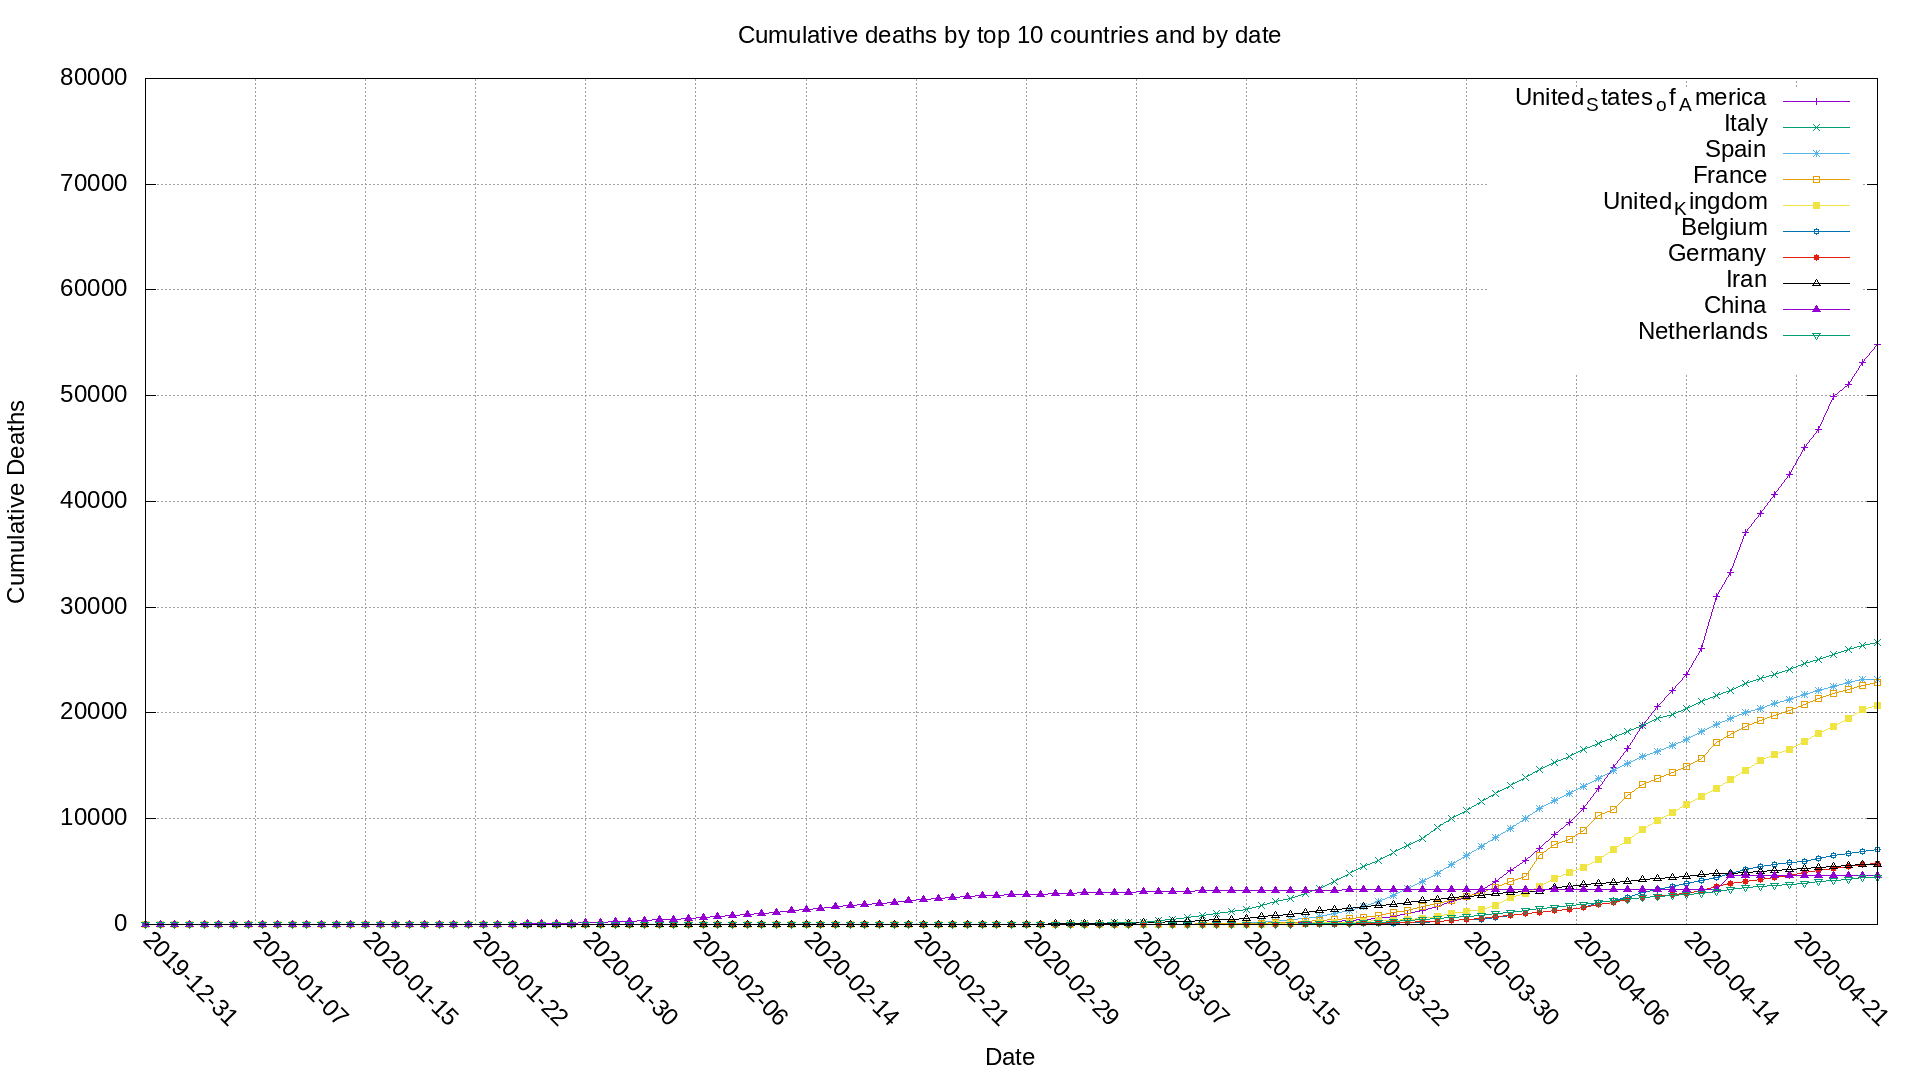
\includegraphics[width=18cm,height=15cm]{graph.png}
    \label{fig:my_label}
\end{figure}


\newpage
\subsection{Derivable functional dependencies from the MINIMAL BASIS} \label{FS}
\begin{multicols}{2}
\begin{itemize}
    \item countriesAndTerritories $\rightarrow$ countryTerritoryCode
    \item countriesAndTerritories $\rightarrow$ continentExp
    \item countriesAndTerritories $\rightarrow$ popData2018
    \item geoId $\rightarrow$ popData2018
    \item dateRep,countriesAndTerritories $\rightarrow$ cases, deaths
    \item day, month, year, geoId $\rightarrow$ cases, deaths
    \item day, month, year, countriesAndTerritories $\rightarrow$ cases, deaths
\end{itemize}
\end{multicols}
\subsection{Further information about EX5} \label{EX5}
\begin{itemize}
    \item 
Definition of partial-key dependency:\\\\
A functional dependency F defined as \textbf{A $\rightarrow$ B} where A is the subset of any candidate key of a relation R and B is a set of non-prime members of R is a partial key dependency.\\
Therefore, the functional dependencies listed in EX5 are partial-key dependencies because the attributes on the right of the FDs are non-prime members and the attributes on the left of the FDs are prime members and proper subsets of a candidate key.
\item A relation R is in the Second Normal Form when:
\begin{itemize}
    \item R is in the First Normal Form
    \item if X is any non-prime attribute of R then X must be fully-functionally dependent on the keys of R. In other words, R cannot contain partial-key dependencies.
\end{itemize}
From the definition above it is possible to gain an understanding of the relational-algebra expressions written in EX5. Indeed, those two expression decompose the Coronavirus relation into two relation so that to eliminate the partial function dependencies present.\\
\item
The algorithm to convert a relation R into Second Normal Form is:
\begin{enumerate}
    \item Collect all candidate keys of R
    \item  Compute the closure of any proper subset X of any key. If there exists a non-prime attribute inside the closure of X then that is an invalidation of the Second Normal Form
    \item Decompose R into R1 and R2 such that\\
    R1=$\Pi_{X \cup \: non-prime \: attributes\: dependent\: on\: X}(R)$\\
    R2=$\Pi_{X \cup \: all \: other \: attributes \: not \: in \: R1}(R)$
    
    \item Recursively repeat steps 1, 2 and 3 for R1 and R2
    
\end{enumerate}
\end{itemize}

\subsection{Further information about EX7} \label{EX7}
Definition of Transitive Functional Dependency:\\
A functional dependency A $\rightarrow$ C is a transitive functional dependency whenever A $\rightarrow$ B, B does not functionally determine A and B $\rightarrow$ C. In other words, a transitive functional dependency occurs in a relation R whenever, given a set of FDs of R, there exists a FD D $\rightarrow$ E  such that D is neither a candidate key nor a super key and E is a set of non-prime attributes.
\subsection{Further information about EX8} \label{EX8}
A relation R is in the Third Normal Form when given that S is the set of FDs of R then for all FDs F A $\rightarrow$ B such that B is a set of non-prime members and F belongs to S then A must be either a key or a super key.\\
The relational-algebra expressions in EX8 decompose the relation Country into two relations so that to eliminate the transitive functional dependency present in the Country relation and obtain two new relations that are in the Third Normal Form.
\subsection{Further information about EX9} \label{EX9}
\begin{itemize}
    \item 
In order to convert the CoronavirusCases relation into the Boyce-Codd-Normal-Form, it must be decomposed into three relations:
\begin{itemize}
    \item CoronavirusCases=$\Pi_{dateRep,cases, deaths, geoId}(CoronavirusCases)$
    \item Dates=$\Pi_{dateRep,day,month,year}(CoronavirusCases)$
    \item CountryTerritory=$\Pi_{geoId, countriesAndTerritories}(CoronavirusCases)$
\end{itemize}
\item The algorithm to convert a relation into the BCNF is:
\begin{enumerate}
    \item Check whether there are FDs of a relation R that violate the BCNF.
    \item If there is a FD X $\rightarrow$ Y that violates the BCNF then compute $\{X\}^{+}$
    \item Decompose R into R1 and R2 such that\\
    R1=$\Pi_{\{X\}^+}(R)$\\
    R2=$\Pi_{X \: \cup \: all \: attributes \: in \: R \: not \: in \:  \{X\}^+}(R)$
    \item Repeat recursively step 1, 2 and 3 for R1 and R2
    
\end{enumerate}
\end{itemize}
\subsection{Further information about EX11} \label{EX11}
\begin{itemize}
    \item 
\textbf{Use of the ”WITHOUT ROWID” keyword:} all the tables have been created by using the ”WITHOUT ROWID” keyword in order to significantly improve the performance of the database. Indeed, by
default, in SQlite the primary key of each table is a UNIQUE SEQUENTIAL INTEGER INDEX. Thus,
even though a user provides a primary key, this one is replaced by this unique index which is called rowid.
This index is stored in a B*-Tree and each node of this tree points to a location in secondary memory where the row
associated with the node's index is located. The real (natural) primary key instead is stored in a B-Tree where
each node's key of this tree is the natural key of a specific tuple and each node’s value is the rowid index the natural key
is associated with. Therefore, retrieving a tuple by using the natural primary key consists of traversing
2 B-trees because firstly the rowid the given primary key value is associated with must be found (B-Tree
traversal) and only after this it is possible to locate the page in secondary memory where the tuple is stored  by traversing the B*-Tree of the indexes. In conclusion, using ”WITHOUT ROWID” leads to retrieval operations which are twice
as fast as the retrieval operations on a table with rowid index. The only disadvantage associated with
”WITHOUT ROWID” is that the primary keys cannot be too large in size. Indeed, it is important to
notice that while the rowid indexes are stored in a B*-Tree (which stores the values in the leaves), the
natural primary keys are stored in a normal B-Tree which stores the values also in the intermediate nodes.
Such a difference could lead to worse performances if the primary keys values were large in size because
every intermediate nodes would take up more space in a single secondary memory page. However, this is
not the case because the primary keys of the relations built for this coursework are not large in size.

\item \textbf{CoronavirusCases relation:} the CoronavirusCases table has been created so that none of its attributes
can be NULL. This choice has been made because otherwise some of the functional dependencies that
have been declared at the beginning of this paper could become not realisable. It is also important to
notice that the primary key of the CoronavirusCases has been declared to be NOT NULL because SQlite
does not prevent a primary key from being NULL automatically. However, other SQL database engines do
this because a primary key CAN NEVER BE NULL. The CoronavirusCases table contains a foreign
key which happens to be also a prime member of the CoronavirusCases relation itself. This foreign key
is the geoId attribute which is the primary key of the CountryContinent table. The attribute geoId is
a foreign key because it is evident that there exists a MANY-TO-ONE RELATIONSHIP from the
CoronavirusCases table to the CountryContinent table. Whenever there exists a many-to-one relationship
from X to Y it is good practice to bring the primary key of Y into X so that the primary key of Y becomes
the foreign key of X and is possible to join the two tables X and Y without a loss of information. This is
why geoId is a foreign key of CoronavirusCases. Some constraints have been applied to geoId so that it is
not possible to delete a row x in the CountryContinent table if a row y of the CoronavirusCases references
x as this would lead to a loss of useful information. Similarly, whenever the attribute geoId is updated
in a row x of the CountryContinet table, the value of the geoId attribute of all rows of CoronavirusCases
that reference to x will be updated as a consequence.
Since, the ”WITHOUT ROWID” keyword has been used then SQlite builds a Clustered Index on the
primary key of the table. This is why the keyword ”ASC” has been used so that all the rows are physically
stored into ascending order with respect to the geoId attribute.
The following additional indexes have been created:
\begin{itemize}
    \item An index on the countriesAndTerritories attribute so that all the queries which involve a select-
from-where (condition on countriesAndTerritories) statements are sped up.
\end{itemize}
There is no need to create an index on the primary key because the primary key is already indexed by
a clustered index. Indeed, the tuples are physically stored into ascending order with respect to the geoId
attribute. For the same reason there is no need of creating an index on geoId. It is important to notice
that no index has been created for the attributes (dateRep, day, month, year, cases, deaths) because the main advantage
of using indexes is to retrieve the position of the tuples that contain a certain attribute value by bringing
into main memory the least number of secondary memory pages as possible (in order to retrieve even a
single tuple from a table, a whole page must be fetched from secondary memory). However, the attributes
(dateRep, day, month, year, cases, deaths) are sparse over most pages (if not all of them).


\item \textbf{CountryContinent relation:} in the CountryContinent relation all attributes, except the primary key geoId, can have null values. Indeed, this can’t cause some functional dependencies to become not realisable. This table contains a foreign key which is the attribute countryterritoryCode. The attribute
countryterritoryCode is the primary key of the CountryPopulation table. Unlike the relationship
between CoronavirusCases and CountryContinent, the relationship between CountryContinent and CountryPopulation is ONE-TO-ONE because every tuple of CountryContinent can reference at most one tuple of the relation CountryPopulation as in the dataset provided not all rows contain a value for the countryterritoryCode attribute. Since, some tuples of the dataset provided contain null values in the countryterritoryCode
attribute and it is the primary key of the relation CountryPopulation then countryterritoryCode must
be a foreign key of the CountryContinent relation. Indeed, if a row x of the CountryContinent relation
contains a non-null value for the attribute countryterritoryCode then it is possible to retrieve the
population of that country by joining the tuple x with the tuple of the CountryPopulation y which has
the same value for the attribute countryterritoryCode. Instead, if a tuple x of the CountryContinet
relation does have a null-value in the countryterritoryCode attribute, then performing the join of this
tuple x with the relation CountryPopulation won’t produce any result because none of the tuples of the
CountryPopulation can have a null value in the countryterritoryCode attribute as it is the primary
key of the relation itself. As regard the index created for this relation, the following have been created:
\begin{itemize}
    \item An index on the countryterritoryCode attribute so that all the queries which involve a select-from-
where (condition on countryterritoryCode) statements are sped up.
\end{itemize}
The geoId attribute is already indexed by the clustered index. It is not convenient to create an index for
the continentExp attribute because the values of this attributes are sparse over many different disk pages
(if not all of them).
\item \textbf{CountryPopulation relation:} the primary key of this relation is the countryterritoryCode attribute
and so it cannot be NULL. On the other hand the popData2018 attribute can have NULL values and
this won’t make any functional dependency not realisable. No indexes have been created in this table
because the primary key is already a clustered index and the popData2018 values are sparse over many disk pages.
\end{itemize}
\subsection{Query operation advantages of the real-life database as shown in the Introduction} \label{EX11Advantages}
The database shown in the introduction section which includes the Countries, Continents and Reports relations does not only represent the data contained in the dataset in a more appropriate way but also makes it possible to speed up some query statements that cannot be optimised in the other database. For example, in the other database it is possible to speed up operations either favouring fast retrieval of tuples by mean of query statements involving the dateRep attribute or by mean of query statements involving the geoId attribute. I have chosen to speed up the retrieval of tuples with respect to the geoId attribute because the final queries involved to write query statements with the geoId as attribute present in the where conditions.
Instead, in the real-life database it is possible to speed up operations for both dateRep and geoId. Indeed, the Reports table can be created by using a clustered index on the primary key which is (dateRep, CountryId). On the other hands, it is possible to create a clustered index on the primary key (ID) of the Countries table. Therefore, the real-life database allows to quickly retrieve information both by date and by country.
\end{document}
